\documentclass[11pt]{article}
\usepackage{spikey}
\usepackage{amsmath}
\usepackage{amssymb}
\usepackage{soul}
\usepackage{float}
\usepackage{graphicx}
\usepackage{hyperref}
\usepackage{xcolor}
\usepackage{chngcntr}
\usepackage{mathrsfs}
\usepackage{centernot}
\usepackage[shortlabels]{enumitem}
\usepackage{verbatim}

\usepackage[margin=1truein]{geometry}
\usepackage{setspace}
\linespread{1.15}

\title{Analysis on PANSS Dataset\\ \small STATS 202: Data Mining and Analysis, Final Project}
\author{Tianyu Du}
\date{\today}

\begin{document}
	\maketitle
	\tableofcontents
	\newpage

	\section{Introduction}
%	\subsection{PANSS Dataset}
	\paragraph{}The Positive and Negative Syndrome Scale (PANSS) score is widely used as a measure for schizophrenia and other disorders in clinical trials. PANSS scores are collected by trained raters and reported by patients or their relatives. One assessment of PANSS scores consists 30 sub-scores from 3 sub-categories: 7 positive scores, 7 negative scores, and 16 general scores. Every score ranges from 1 to 7 denoting increasing levels of psychopathology. The aggregation of all 30 scores provides a detailed assessment of patient's current psychological status.
	
	\paragraph{}The entire dataset consists of five different studies ranging from study A to study E. In this practice, the first four datasets are used as a training to fit, select, and evaluate models. Then, these selected models are used to recover missing data in study E.
	
	\section{Treatment Effects}
	\paragraph{}This section is devoted to analyze whether the treatment assigned leads to significant improvements on patients' psychological status. Because the 18-th week assessments are missing in the dataset of study E, in this section, only data from study A to D are considered. There are 20947 observations (assessments) from above-mentioned dataset, in which 10524 observations came from patients assigned to the control group, and the remaining 10423 were from participants belonged to the treatment group. The evenly-split dataset allows us to deploy various models to analyze whether there exists significant treatment effects.
	
	\paragraph{}Multiple evidences were found to support that there were indeed no treatment effect in this study. Firstly, the effects on four aggregate scores are analyzed, namely sum of all PANSS scores, and sums of scores from positive (\texttt{P\_Total}), negative (\texttt{N\_Total}), and general (\texttt{G\_Total}) sub-categories respectively.
	
	\paragraph{}One challenge associated with treatment effect analysis is the initial status of patients in different groups.
	Figure 1 below presents the distributions of the four aggregate scores at day 0 visit. 	The figure suggested similar distributions were shared among the treatment and control groups.
	
	\begin{figure}[h]
		\centering
		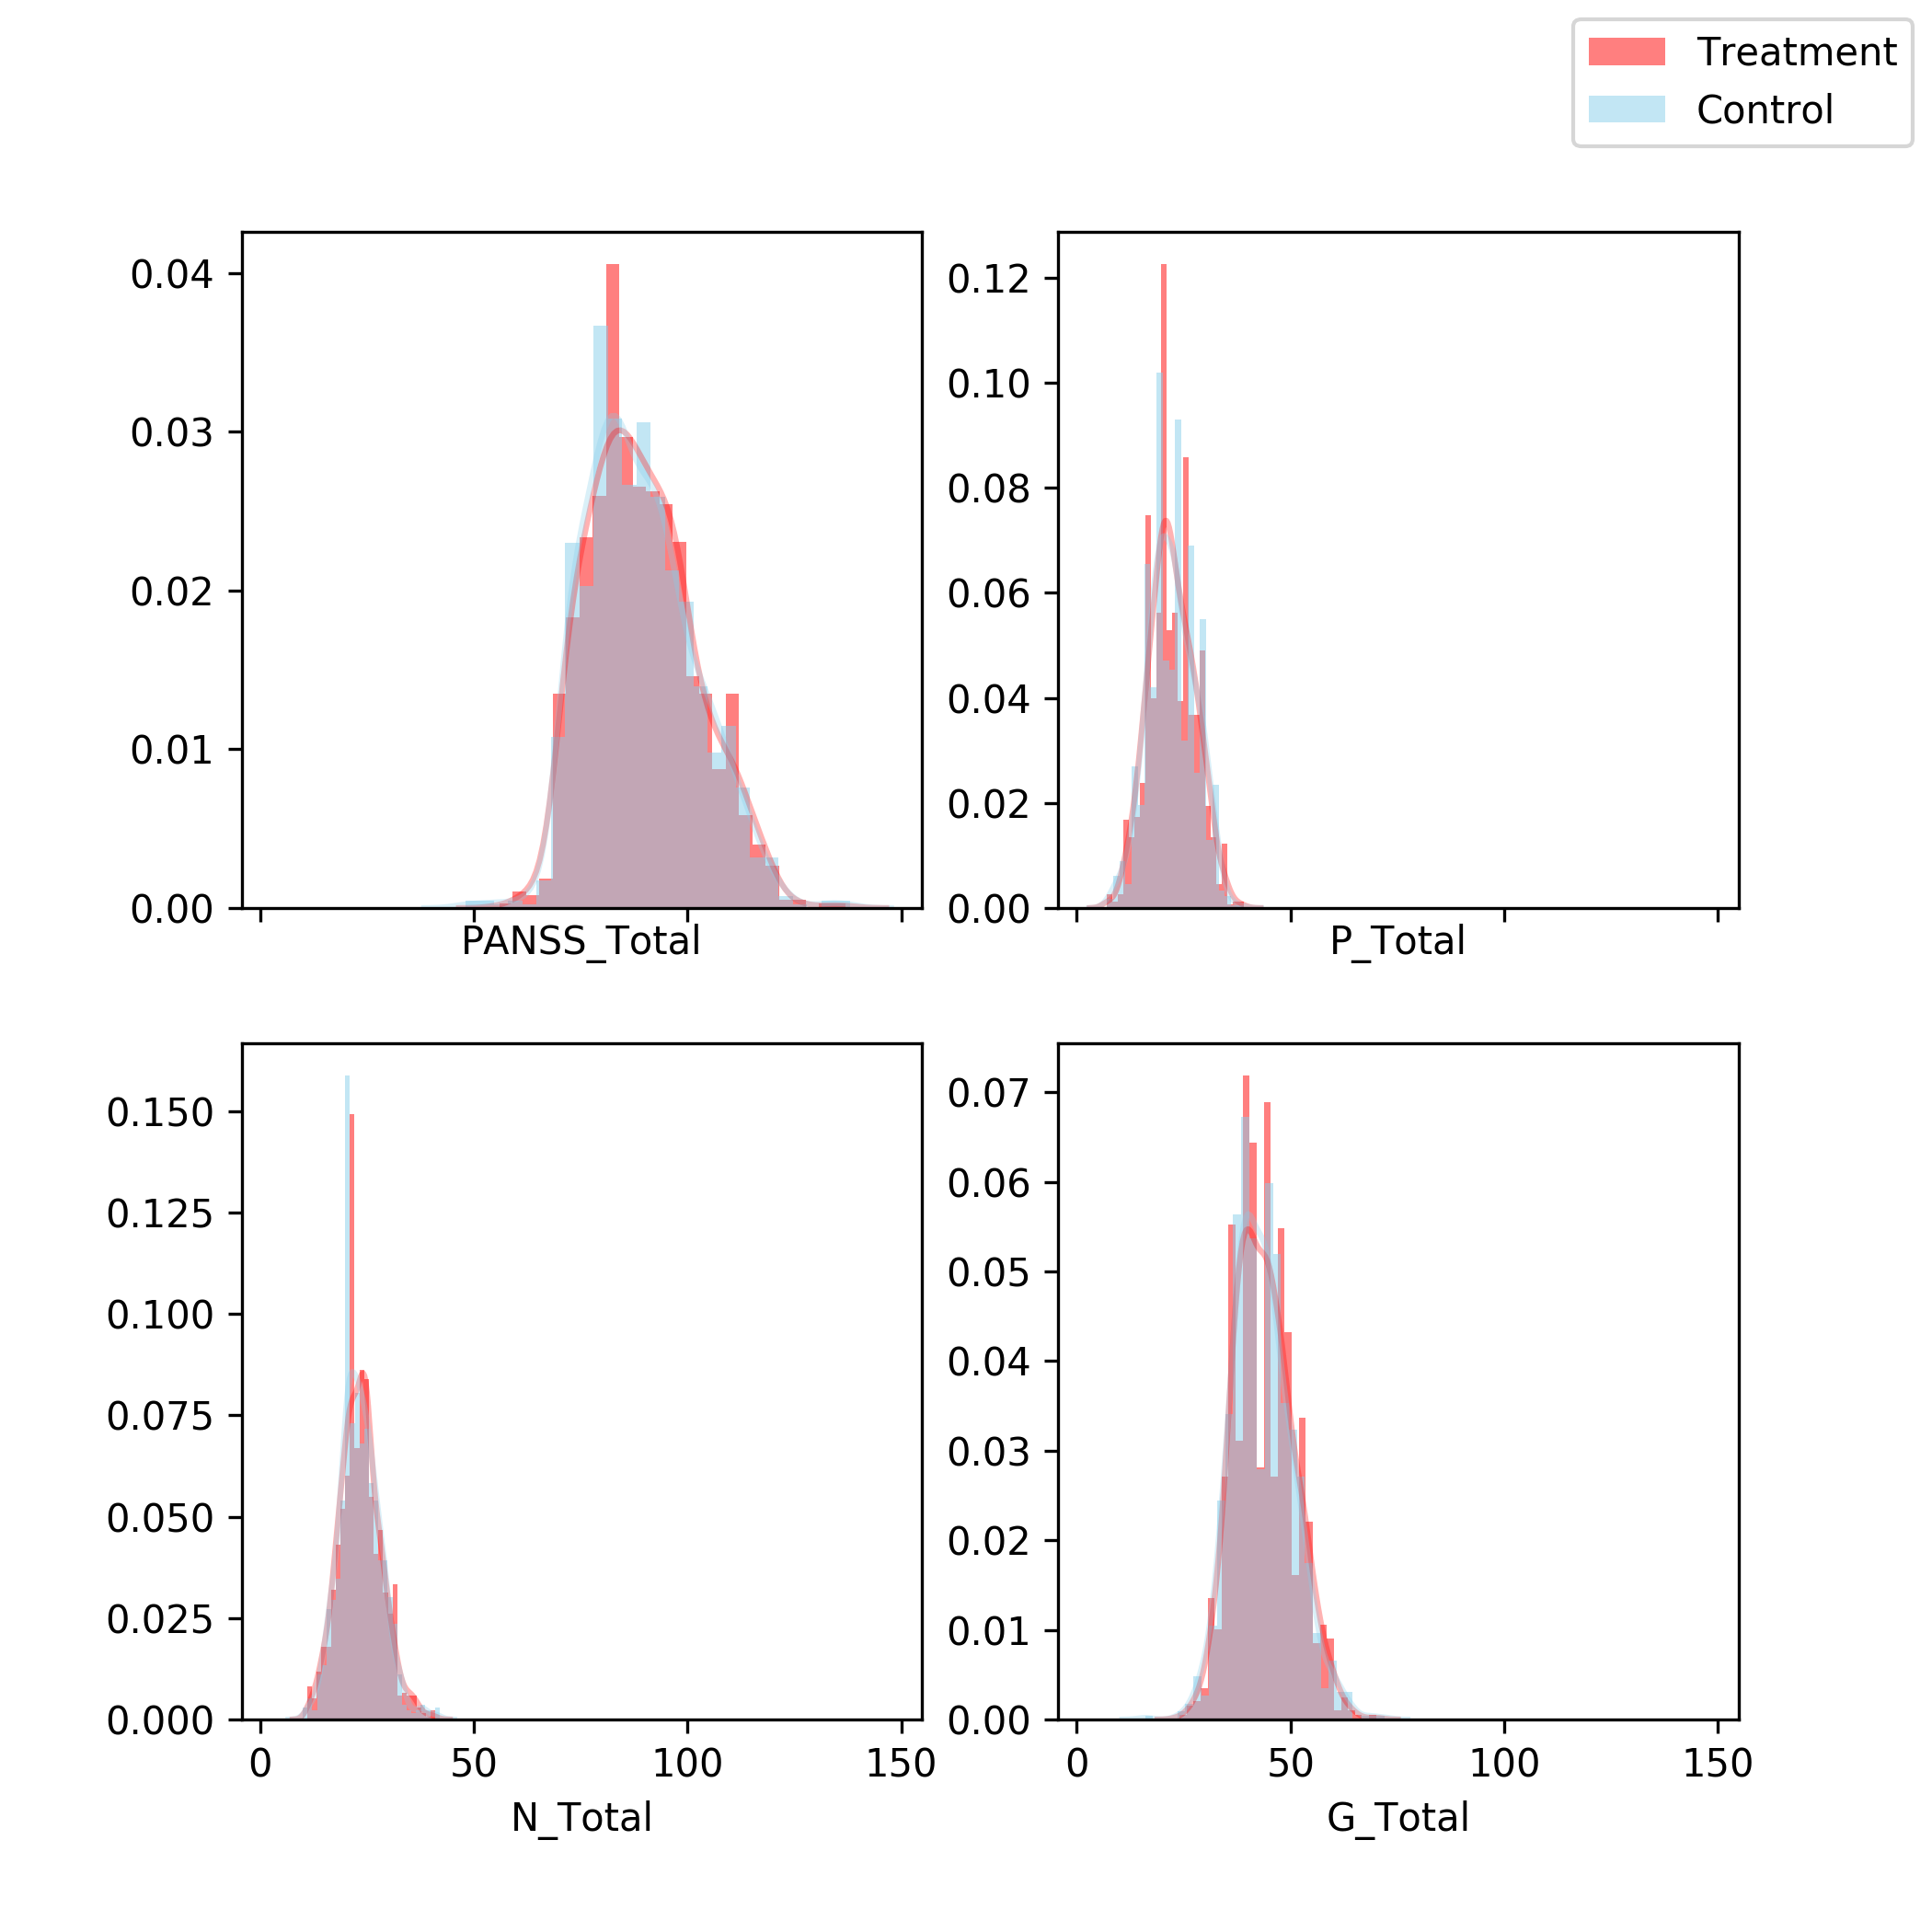
\includegraphics[width=0.7\linewidth]{figures/dist_initial_scores.png}
		\caption{Distributions of Aggregate Scores at Day 0}
	\end{figure}
	
	\section{Patient Segmentation}
	\section{Patient PANSS Forecasting}
	\section{Assessment Validity Classification}
\end{document}










